\subsubsection{Туннельный диод}

\begin{center}
	\begin{figure}[h!]
		\center{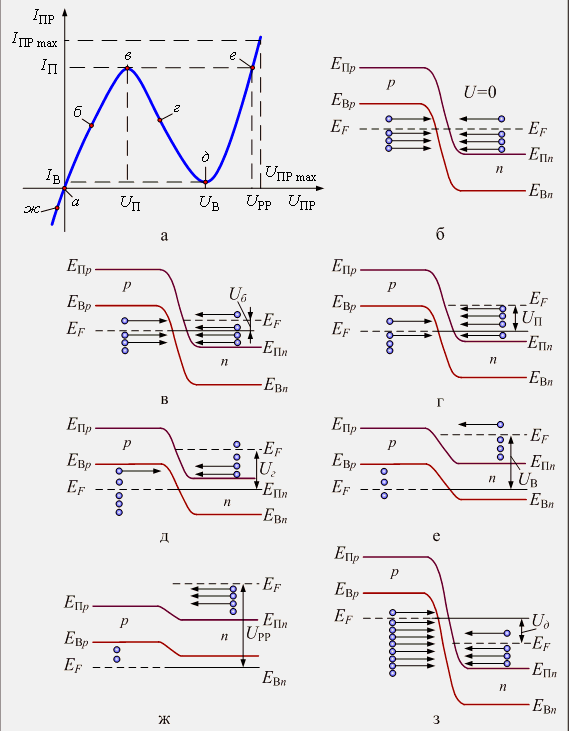
\includegraphics[scale=0.9]{TunnelDiod.png}}
		\caption{ВАХ и энергетические диаграммы при различных смещениях}	
		\label{pic:TunnelDiod}
	\end{figure}
\end{center}

Туннельный диод выполнен из двух сильно легированных n и p слоев. Эти слои легированы так сильно, что уровень ферми лежит не в запрещенной зоне, а в зоне проводимости для n-типа и в валентной зоне для p-типа.
Ширина pn-перехода также крайне мала у таких диодов, что приводит к появлению туннельного эффекта.
При подаче обратного напряжения на диод количество электронов, энергия которых превышает уровень Ферми в n-слое не возрастет, а в p-слое возрастет и следовательно электроны будут туннелировать из p  слоя в n, что соответствует току из n в p. 

При включении прямого напряжение начальное возрастание тока обусловлено теми же причинами, которыми обусловлено его наличие при обратном включении, но только до той степени, пока энергетические зоны окончательно не разъехались. После этого диод начинает работать как обычный.


 Так как возникновение туннельного тока нес вязано с инжекцией носителей заряда, туннельные диоды имеют малую инерционность и вследствие этого могут применяться для усиления и генерации высокочастотных колебаний.



